% !TeX program = xelatex
\documentclass[a4paper,14pt]{article}

% --- Настройка шрифтов и локализации для XeLaTeX (с запасными шрифтами) ---
% \usepackage{fontspec}
% \usepackage{polyglossia}
% \setmainlanguage{russian}
% \setotherlanguage{english}
% \defaultfontfeatures{Ligatures=TeX}
% \IfFontExistsTF{Times New Roman}{\setmainfont{Times New Roman}}
%   {\IfFontExistsTF{Liberation Serif}{\setmainfont{Liberation Serif}}
%   {\setmainfont{TeX Gyre Termes}}}
% \IfFontExistsTF{Courier New}{\setmonofont{Courier New}}
%   {\IfFontExistsTF{Liberation Mono}{\setmonofont{Liberation Mono}}
%   {\setmonofont{DejaVu Sans Mono}}}

\usepackage{fontspec}
\usepackage{xunicode}
\usepackage{xltxtra}
\usepackage{polyglossia}
\setmainlanguage{russian}
\setotherlanguage{english}
\defaultfontfeatures{Ligatures=TeX}
\setmainfont{Times New Roman}
\newfontfamily\cyrillicfont{Times New Roman}
\setmonofont{Courier New}
\newfontfamily\cyrillicfonttt{Courier New}

% --- Параметры страницы по ГОСТ (левое 3 см, правое 1 см, верхнее и нижнее по 2 см) ---
\usepackage[left=30mm, right=10mm, top=20mm, bottom=20mm]{geometry}

% --- Интервалы и абзацный отступ (1.25 см, 1.5 интервал) ---
\usepackage{indentfirst}
\setlength{\parindent}{1.25cm}
\usepackage{setspace}
\onehalfspacing

% --- Пакеты для таблиц, списков и графики ---
\usepackage{tabularx}
\usepackage{booktabs}
\usepackage{array}
\usepackage{enumitem}
\setlist{nosep, leftmargin=\parindent}
\usepackage{graphicx}

% --- Листинги SQL ---
\usepackage{listings}
\usepackage{xcolor}

\lstset{
    basicstyle=\ttfamily\footnotesize,
    columns=flexible,
    keepspaces=true,
    breaklines=true,
    frame=single,
    tabsize=2,
    showstringspaces=false,
    keywordstyle=\bfseries\color{blue!70!black},
    commentstyle=\itshape\color{green!50!black},
    stringstyle=\color{red!60!black},
    numbers=none,
    language=SQL
}

% --- Оформление заголовков по стандарту ---
\usepackage{titlesec}
\titleformat{\section}[block]
  {\normalfont\bfseries\filright}
  {\hspace{1.25cm}\thesection\quad}
  {0pt}
  {\MakeUppercase}

\titleformat{\subsection}[block]
  {\normalfont\bfseries\filright}
  {\hspace{1.25cm}\thesubsection\quad}
  {0pt}
  {}

\titlespacing*{\section}{0pt}{18pt}{12pt}
\titlespacing*{\subsection}{0pt}{12pt}{6pt}

% --- Подписи к рисункам и таблицам ---
\usepackage[tableposition=top,figureposition=bottom]{caption}
\DeclareCaptionLabelSeparator{emdash}{~---~}
\captionsetup[figure]{
  name={Рисунок},
  labelsep=emdash,
  font={small},
  justification=centering,
  singlelinecheck=true
}
\captionsetup[table]{
  name={Таблица},
  labelsep=emdash,
  font={small},
  justification=raggedright,
  singlelinecheck=false
}

% --- Отточие в содержании ---
\usepackage{tocloft}
\renewcommand{\cftsecleader}{\cftdotfill{\cftdotsep}}
\renewcommand{\cfttoctitlefont}{\hfill\bfseries\MakeUppercase}
\renewcommand{\cftaftertoctitle}{\hfill}

% --- Рисунок, который может ещё отсутствовать: вместо него выводится рамка-заглушка ---
\newcommand{\optfigure}[3]{% файл, ширина, текст заглушки
  \IfFileExists{#1}
    % {\includegraphics[width=#2]{#1}}
    {\fbox{\parbox{0.8\textwidth}{\centering\vspace{1.5em}\textbf{[Вставьте скриншот]}\\ #3\vspace{1.5em}}}}%
}

\begin{document}

% =========================================================================
% ТИТУЛЬНЫЙ ЛИСТ
% =========================================================================
\begin{titlepage}
    \centering
    {\small МИНИСТЕРСТВО НАУКИ И ВЫСШЕГО ОБРАЗОВАНИЯ РОССИЙСКОЙ ФЕДЕРАЦИИ}\\
    {\scriptsize \textbf{ФЕДЕРАЛЬНОЕ ГОСУДАРСТВЕННОЕ АВТОНОМНОЕ ОБРАЗОВАТЕЛЬНОЕ УЧРЕЖДЕНИЕ ВЫСШЕГО ОБРАЗОВАНИЯ}}\\
    {\bfseries «НАЦИОНАЛЬНЫЙ ИССЛЕДОВАТЕЛЬСКИЙ УНИВЕРСИТЕТ ИТМО»}\\[0.8cm]

    \textbf{Факультет безопасности информационных технологий}\\[0.6cm]

    \textbf{Направление подготовки: 10.03.01 Информационная безопасность} \\
    \textbf{Образовательная программа: «Технологии защиты информации»} \\[0.6cm]

    \textbf{Дисциплина:} \\
    \textit{\textbf{«Информационная безопасность баз данных»}} \\ [1.5cm]

    {\bfseries ОТЧЕТ ПО ЛАБОРАТОРНОЙ РАБОТЕ №3}\\
    \textit{{\bfseries «Разработка примитивной системы защиты на уровне СУБД»}}\\[4cm]

    \begin{flushright}
        \textbf{Выполнил студент(ы):} \\ [0.5em]
        группа.поток ИББД 1.7 \\ [0.5em]
        Пахомов Владимир Юрьевич / \raisebox{-0.3\height}{
\includegraphics[width=1.3cm]{sign1.png}} \\
        {\scriptsize{\textit{ФИО \hspace{2cm} Подпись \hspace{0.3cm}}}} \\ [0.3cm]
        Сивков Иван Александрович / \raisebox{-0.4\height}{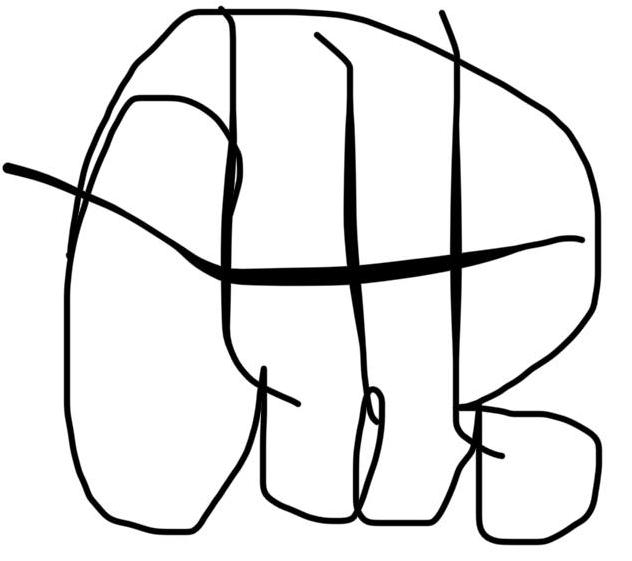
\includegraphics[width=1.1cm]{sign2.jpg}} \\
        {\scriptsize{\textit{ФИО \hspace{2cm} Подпись \hspace{0.3cm}}}} \\ [0.3cm]
        Булин Михаил Михайлович / \raisebox{-0.4\height}{
\includegraphics[width=1.3cm]{sign3.png}} \\
        {\scriptsize{\textit{ФИО \hspace{2cm} Подпись \hspace{0.3cm}}}} \\ [0.3cm]


        \textbf{Проверил:}\\ [0.5em]
        Ярцева Наталия Андреевна / \underline{\hspace{1.5cm}} \\
        {\scriptsize{\textit{ФИО \hspace{2cm} Подпись \hspace{1cm}}}} \\ [1.5cm]

        {\scriptsize \underline{\hspace{4cm}}} \\
        {\scriptsize \textit{Отметка о выполнении (один из вариантов: \\ отлично, хорошо, удовлетворительно, зачтено)}} \\
        {\scriptsize \underline{\hspace{4cm}}} \\
        {\scriptsize \textit{Дата \hspace{1.5cm}}}
    \end{flushright}


    \vfill
    Санкт-Петербург\\
    2026
\end{titlepage}

% =========================================================================
% СОДЕРЖАНИЕ
% =========================================================================
\newpage
\pagestyle{plain}
\setcounter{page}{2}

\begin{center}
    {\bfseries \MakeUppercase{Содержание}}
\end{center}
\vspace{-0.5cm}
\tableofcontents

% =========================================================================
% ВВЕДЕНИЕ
% =========================================================================
\newpage
\begin{center}
    {\bfseries \MakeUppercase{Введение}}
\end{center}
\addcontentsline{toc}{section}{ВВЕДЕНИЕ}

\textbf{Цель работы}: получение навыков создания примитивных систем мониторинга, разграничения доступа и шифрования средствами СУБД.

Объектом защиты выступает база данных \texttt{container\_cargo\_db} информационной системы морских контейнерных перевозок, спроектированная в лабораторной работе №1. База данных включает 9 отношений (\textit{clients}, \textit{ports}, \textit{ships}, \textit{containers}, \textit{orders}, \textit{voyages}, \textit{invoices}, \textit{order\_containers}, \textit{voyage\_orders}) и 4 представления для двух классов потребителей информации: «Клиент / Грузоотправитель» и «Диспетчер флота / Логист терминала». Реализация выполняется в СУБД PostgreSQL с использованием расширения \textit{pgcrypto}.

В работе решаются три задачи: мониторинг изменений данных с помощью триггеров и таблицы-лога, шифрование таблицы с секретными данными симметричным алгоритмом AES-256 и разграничение доступа на основе ролей по принципу наименьших привилегий.

% =========================================================================
% 1. МОНИТОРИНГ
% =========================================================================
\newpage
\section{Задачи по мониторингу операций в БД}

\subsection{Таблица-лог и триггерная функция}
Создадим таблицу-лог \texttt{main\_log}, отдельную от основных сущностей базы данных. Для каждой зарегистрированной операции в ней сохраняются тип операции, имя таблицы, время выполнения, роль, от лица которой поступил запрос, а также старые и новые значения изменяемого кортежа в формате JSON. Атрибут \texttt{log\_item\_id} является автогенерируемым идентификатором записи.

\begin{lstlisting}
CREATE TABLE IF NOT EXISTS public.main_log (
    log_item_id    integer GENERATED BY DEFAULT AS IDENTITY PRIMARY KEY, -- автоинкремент
    operation_type text        NOT NULL,                                 -- I / U / D
    table_name     text        NOT NULL,                                 -- в какой таблице изменение
    operation_date timestamptz NOT NULL DEFAULT now(),                   -- когда
    user_operator  text        NOT NULL,                                 -- активная роль (current_user)
    session_login  text        NOT NULL,                                 -- роль входа в сессию (session_user)
    old_data       jsonb,                                                -- старые значения (U, D)
    new_data       jsonb                                                 -- новые значения (I, U)
);
\end{lstlisting}

Создадим триггерную функцию \texttt{logging()}, которая срабатывает при изменениях данных и заносит в таблицу-лог информацию об операции. Для вставки фиксируются только новые значения, для удаления~--- только старые, для изменения~--- и старые, и новые. Роль, выполнившая запрос, определяется функциями \texttt{current\_user} (активная роль) и \texttt{session\_user} (роль, под которой выполнен вход в сессию).

\begin{lstlisting}
CREATE OR REPLACE FUNCTION public.logging() RETURNS trigger AS $logging$
BEGIN
    IF (TG_OP = 'INSERT') THEN
        INSERT INTO public.main_log (operation_type, table_name, user_operator, session_login, old_data, new_data)
        VALUES ('I', TG_TABLE_NAME, current_user, session_user, NULL, to_jsonb(NEW)); -- вставка: только новые
    ELSIF (TG_OP = 'UPDATE') THEN
        INSERT INTO public.main_log (operation_type, table_name, user_operator, session_login, old_data, new_data)
        VALUES ('U', TG_TABLE_NAME, current_user, session_user, to_jsonb(OLD), to_jsonb(NEW)); -- изменение: старые и новые
    ELSIF (TG_OP = 'DELETE') THEN
        INSERT INTO public.main_log (operation_type, table_name, user_operator, session_login, old_data, new_data)
        VALUES ('D', TG_TABLE_NAME, current_user, session_user, to_jsonb(OLD), NULL); -- удаление: только старые
    END IF;
    RETURN NULL; -- для AFTER-триггера возвращаемое значение не важно
END;
$logging$ LANGUAGE plpgsql;
\end{lstlisting}

\subsection{Создание триггеров для основных таблиц}
Для каждой из девяти основных таблиц создадим триггер \texttt{logging\_exec}, который вызывает функцию \texttt{logging()} после любой вставки, изменения или удаления кортежа. Триггер объявлен как построчный (\texttt{FOR EACH ROW}), поэтому каждое изменённое кортеж-значение фиксируется отдельной записью в логе. Чтобы не дублировать однотипные команды, триггеры создаются в цикле:

\begin{lstlisting}
DO $$
DECLARE t text;
BEGIN
    FOREACH t IN ARRAY ARRAY['clients', 'ports', 'ships', 'containers', 'orders',
                             'voyages', 'invoices', 'order_containers', 'voyage_orders'] LOOP
        EXECUTE format(
            'CREATE OR REPLACE TRIGGER logging_exec AFTER INSERT OR UPDATE OR DELETE ON public.%I FOR EACH ROW EXECUTE FUNCTION public.logging()',
            t);
    END LOOP;
END $$;
\end{lstlisting}

Для одной таблицы эквивалентная команда имеет вид:

\begin{lstlisting}
CREATE TRIGGER logging_exec
AFTER INSERT OR UPDATE OR DELETE ON clients
FOR EACH ROW EXECUTE FUNCTION logging();
\end{lstlisting}

\subsection{Демонстрация работы системы логирования}
Продемонстрируем работу системы для различных операций и отношений. Для наглядности выполним операции над двумя таблицами~--- \textit{ports} и \textit{clients}: вставим по одному кортежу, изменим их и удалим. Работа выполняется над собственными тестовыми строками, чтобы не нарушать ограничения внешних ключей.

\begin{lstlisting}
INSERT INTO public.ports (name, country, dock_count, max_draft)
VALUES ('Test Port', 'Russia', 5, 12.5);                                       -- INSERT

INSERT INTO public.clients (name, email, phone, address)
VALUES ('Test Cargo LLC', 'old@test.ru', '+70000000000', 'Saint Petersburg');  -- INSERT

UPDATE public.clients SET email = 'new@test.ru' WHERE name = 'Test Cargo LLC'; -- UPDATE

UPDATE public.ports SET dock_count = 8 WHERE name = 'Test Port';               -- UPDATE

DELETE FROM public.clients WHERE name = 'Test Cargo LLC';                      -- DELETE
DELETE FROM public.ports WHERE name = 'Test Port';                             -- DELETE

SELECT * FROM public.main_log ORDER BY log_item_id;
\end{lstlisting}

Содержимое таблицы-лога после выполнения операций приведено на рисунке \ref{fig:log}.

\begin{figure}[h!]
    \centering
    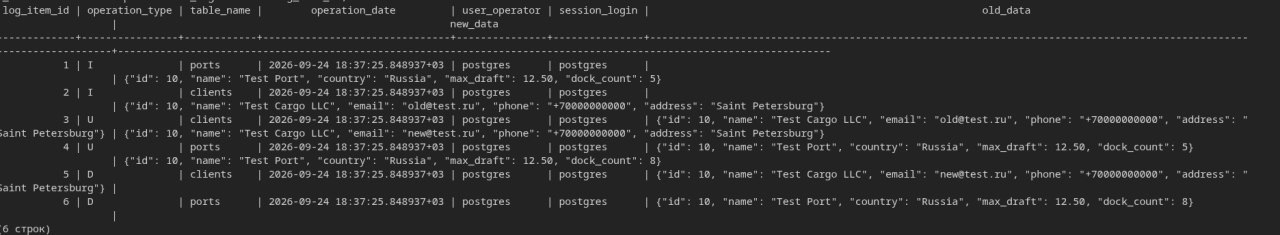
\includegraphics[width=\textwidth]{fig_log.jpg}
    \caption{Логирование операций вставки, изменения и удаления}
    \label{fig:log}
\end{figure}

В таблице зафиксировано шесть записей. Записи 1 и 2 (тип \texttt{I}) соответствуют вставке в таблицы \textit{ports} и \textit{clients}: заполнено только поле \texttt{new\_data}. Записи 3 и 4 (тип \texttt{U}) соответствуют изменению: в них сохранены и старые, и новые значения (например, адрес электронной почты клиента изменён с \texttt{old@test.ru} на \texttt{new@test.ru}, число причалов порта~--- с 5 на 8). Записи 5 и 6 (тип \texttt{D}) соответствуют удалению: заполнено только поле \texttt{old\_data}. Во всех записях указаны время операции и роль (\texttt{postgres}), от лица которой выполнен запрос.

% =========================================================================
% 2. ШИФРОВАНИЕ
% =========================================================================
\newpage
\section{Задачи по шифрованию данных}

\subsection{Таблица с секретными данными}
Создадим таблицу \texttt{secret\_data}, отдельную от основных сущностей. В ней хранятся токены доступа пользователей информационной системы. Оба содержательных столбца имеют тип \texttt{bytea}, так как результатом шифрования является двоичная строка.

\begin{lstlisting}
CREATE EXTENSION IF NOT EXISTS pgcrypto;

CREATE TABLE IF NOT EXISTS public.secret_data (
    id           integer GENERATED BY DEFAULT AS IDENTITY PRIMARY KEY,
    username     bytea, -- шифртекст (pgp_sym_encrypt возвращает bytea)
    secret_token bytea
);
\end{lstlisting}

\subsection{Формирование ключа и шифрование содержимого}
Для шифрования используется симметричный алгоритм AES-256 (функция \texttt{pgp\_sym\_encrypt} расширения \textit{pgcrypto} с параметром \texttt{cipher-algo=aes256}). Ключ шифрования в информационной системе не хранится: он вычисляется как значение детерминированной хэш-функции SHA-256 от индивидуального пароля суперпользователя. Этот пароль не связан с паролем для входа в СУБД и известен только суперпользователю. Таким образом, без знания пароля восстановить ключ (и, следовательно, расшифровать данные) невозможно, поскольку хэш-функция является односторонней.

Пусть индивидуальным паролем суперпользователя будет \texttt{personal\_admin\_pass}. Вставим данные в зашифрованном виде; ключ вычисляется непосредственно в запросе и нигде не сохраняется:

\begin{lstlisting}
INSERT INTO public.secret_data (username, secret_token)
SELECT pgp_sym_encrypt(v.u, k.key, 'cipher-algo=aes256'),  -- AES-256
       pgp_sym_encrypt(v.t, k.key, 'cipher-algo=aes256')
FROM (VALUES ('shipper_ivanov',    'token_4fsdf43fdaf43r2fdsa'),
             ('dispatcher_petrov', 'token_13gdfss4fa232fdsadfsa')) AS v(u, t),
     (SELECT encode(digest('personal_admin_pass', 'sha256'), 'hex') AS key) AS k;
\end{lstlisting}

Функция \texttt{pgp\_sym\_encrypt} при каждом вызове использует случайную соль, поэтому одинаковые открытые значения дают различающийся шифртекст.

\subsection{Демонстрация невозможности чтения без пароля}
Выведем содержимое таблицы. Даже пользователь с правом чтения таблицы (в том числе администратор) видит только шифртекст (рисунок \ref{fig:secret}).

\begin{lstlisting}
SELECT * FROM public.secret_data;
\end{lstlisting}

% \begin{figure}[h!]
%     \centering
%     \optfigure{fig_secret_table.png}{0.9\textwidth}{Результат запроса \texttt{SELECT * FROM public.secret\_data;} (в столбцах должен быть шифртекст типа bytea)}
%     \caption{Содержимое таблицы «secret\_data» в зашифрованном виде}
%     \label{fig:secret}
% \end{figure}

\begin{figure}[h!]
    \centering
    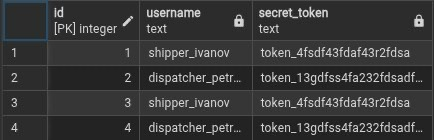
\includegraphics[width=0.7\textwidth]{fig_secret_table.png}
    \caption{Содержимое таблицы «secret\_data» в зашифрованном виде}
    \label{fig:secret}
\end{figure}

Расшифровка выполняется только при указании ключа, полученного из верного индивидуального пароля:

\begin{lstlisting}
SELECT id,
       pgp_sym_decrypt(username,     encode(digest('personal_admin_pass', 'sha256'), 'hex')) AS username,
       pgp_sym_decrypt(secret_token, encode(digest('personal_admin_pass', 'sha256'), 'hex')) AS secret_token
FROM public.secret_data;
\end{lstlisting}

При попытке расшифровать данные с неверным паролем СУБД возвращает ошибку (рисунок \ref{fig:wrongkey}):

\begin{lstlisting}
SELECT pgp_sym_decrypt(secret_token, encode(digest('wrong_pass', 'sha256'), 'hex'))
FROM public.secret_data;
\end{lstlisting}

\begin{figure}[h!]
    \centering
    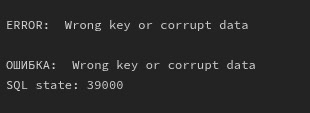
\includegraphics[width=0.45\textwidth]{fig_wrong_key.jpg}
    \caption{Попытка расшифровки с неверным ключом}
    \label{fig:wrongkey}
\end{figure}

Следовательно, обладание правами администратора без знания индивидуального пароля не позволяет получить содержимое таблицы с секретными данными.

% =========================================================================
% 3. РАЗГРАНИЧЕНИЕ ДОСТУПА
% =========================================================================
\newpage
\section{Задачи по разграничению доступа в БД}

\subsection{Групповые роли для классов потребителей}
Согласно системному анализу (ЛР1), в системе выделены два класса потребителей информации: «Клиент / Грузоотправитель» и «Диспетчер флота / Логист терминала». Для каждого из них создадим групповую роль без права входа. Дополнительно создадим групповую роль «Админ», которая должна иметь возможность просматривать все таблицы и представления базы данных.

\begin{lstlisting}
CREATE ROLE client_group_role     NOLOGIN NOSUPERUSER NOCREATEDB NOCREATEROLE INHERIT; -- Клиент / Грузоотправитель
CREATE ROLE dispatcher_group_role NOLOGIN NOSUPERUSER NOCREATEDB NOCREATEROLE INHERIT; -- Диспетчер / Логист
CREATE ROLE admin_group_role      NOLOGIN NOSUPERUSER NOCREATEDB NOCREATEROLE INHERIT; -- Админ
\end{lstlisting}

\subsection{Назначение привилегий групповым ролям}
Привилегии назначаются по принципу наименьших привилегий: каждой группе предоставляется доступ на чтение только к тем представлениям, которые необходимы ей для решения задач, определённых в ЛР1. Прямой доступ к базовым таблицам потребителям не предоставляется. Таблица логирования доступна только суперпользователю. Сводка привилегий приведена в таблице \ref{tab:privs}.

\begin{table}[h!]
    \caption{Привилегии групповых ролей}
    \label{tab:privs}
    \small
    \begin{tabularx}{\textwidth}{|l|X|}
        \hline
        \textbf{Групповая роль}          & \textbf{Доступные объекты (SELECT)}                                                    \\ \hline
        \textit{client\_group\_role}     & представления \textit{view\_client\_orders}, \textit{view\_client\_tracking}           \\ \hline
        \textit{dispatcher\_group\_role} & представления \textit{view\_voyage\_manifest}, \textit{view\_container\_safety\_audit} \\ \hline
        \textit{admin\_group\_role}      & все 9 таблиц основной схемы, таблица \textit{secret\_data}, все 4 представления        \\ \hline
        \textit{main\_log}               & только суперпользователь                                                               \\ \hline
    \end{tabularx}
\end{table}

\begin{lstlisting}
-- Клиент: только свои представления из ЛР1
GRANT SELECT ON TABLE public.view_client_orders   TO client_group_role;
GRANT SELECT ON TABLE public.view_client_tracking TO client_group_role;

-- Диспетчер: только свои представления из ЛР1
GRANT SELECT ON TABLE public.view_voyage_manifest        TO dispatcher_group_role;
GRANT SELECT ON TABLE public.view_container_safety_audit TO dispatcher_group_role;

-- Админ: все таблицы и представления, кроме лога (лог видит только суперпользователь)
GRANT SELECT ON TABLE
    public.clients, public.ports, public.ships, public.containers, public.orders,
    public.voyages, public.invoices, public.order_containers, public.voyage_orders,
    public.secret_data,
    public.view_client_orders, public.view_client_tracking,
    public.view_voyage_manifest, public.view_container_safety_audit
TO admin_group_role;
\end{lstlisting}

\subsection{Индивидуальные роли пользователей}
Создадим по одному пользователю для каждой групповой роли (с правом входа) и включим их в соответствующие группы:

\begin{lstlisting}
CREATE ROLE shipper_ivanov    WITH LOGIN PASSWORD 'change_me_1' NOSUPERUSER NOCREATEDB NOCREATEROLE;
CREATE ROLE dispatcher_petrov WITH LOGIN PASSWORD 'change_me_2' NOSUPERUSER NOCREATEDB NOCREATEROLE;
CREATE ROLE admin_sidorov     WITH LOGIN PASSWORD 'change_me_3' NOSUPERUSER NOCREATEDB NOCREATEROLE;

GRANT client_group_role     TO shipper_ivanov;
GRANT dispatcher_group_role TO dispatcher_petrov;
GRANT admin_group_role      TO admin_sidorov;
\end{lstlisting}

\subsection{Проверка работы системы разграничения доступа}
Для проверки войдём под каждой из индивидуальных ролей с помощью команды \texttt{SET ROLE} и обратимся к отношениям базы данных. После проверки возврат к исходной роли выполняется командой \texttt{RESET ROLE}.

\textbf{Роль «shipper\_ivanov» (Клиент).} Доступны только представления \textit{view\_client\_orders} и \textit{view\_client\_tracking}; обращение к остальным объектам завершается ошибкой \texttt{permission denied}.

\begin{lstlisting}
SET ROLE shipper_ivanov;
SELECT * FROM public.view_client_orders;          -- OK
SELECT * FROM public.view_client_tracking;        -- OK
SELECT * FROM public.view_voyage_manifest;        -- permission denied
SELECT * FROM public.orders;                      -- permission denied
SELECT * FROM public.secret_data;                 -- permission denied
SELECT * FROM public.main_log;                    -- permission denied
RESET ROLE;
\end{lstlisting}

\textbf{Роль «dispatcher\_petrov» (Диспетчер).} Доступны только представления \textit{view\_voyage\_manifest} и \\ \textit{view\_container\_safety\_audit}.

\begin{lstlisting}
SET ROLE dispatcher_petrov;
SELECT * FROM public.view_voyage_manifest;        -- OK
SELECT * FROM public.view_container_safety_audit; -- OK
SELECT * FROM public.view_client_orders;          -- permission denied
SELECT * FROM public.clients;                     -- permission denied
SELECT * FROM public.secret_data;                 -- permission denied
RESET ROLE;
\end{lstlisting}

\textbf{Роль «admin\_sidorov» (Админ).} Доступны все таблицы и представления, кроме таблицы логирования. Содержимое таблицы \textit{secret\_data} видно только в зашифрованном виде: расшифровка без индивидуального пароля завершается ошибкой.

\begin{lstlisting}
SET ROLE admin_sidorov;
SELECT * FROM public.orders;                      -- OK
SELECT * FROM public.secret_data;                 -- OK, но только шифртекст
SELECT pgp_sym_decrypt(secret_token, encode(digest('guess', 'sha256'), 'hex'))
FROM public.secret_data;                          -- ошибка: Wrong key or corrupt data
SELECT * FROM public.main_log;                    -- permission denied
RESET ROLE;
\end{lstlisting}

% =========================================================================
% ЗАКЛЮЧЕНИЕ
% =========================================================================
\newpage
\begin{center}
    {\bfseries \MakeUppercase{Заключение}}
\end{center}
\addcontentsline{toc}{section}{ЗАКЛЮЧЕНИЕ}

В ходе выполнения лабораторной работы для базы данных «Информационная система морских контейнерных перевозок» была разработана примитивная система защиты на уровне СУБД PostgreSQL.

В рамках работы были достигнуты следующие результаты:
\begin{enumerate}
    \item Создана таблица-лог \texttt{main\_log} и триггерная функция \texttt{logging()}. Для всех девяти основных таблиц созданы триггеры, фиксирующие вставку, изменение и удаление кортежей с указанием времени, роли и старых и новых значений. Работа системы продемонстрирована на нескольких таблицах и типах операций.
    \item Создана таблица \texttt{secret\_data} с секретными данными, содержимое которой зашифровано алгоритмом AES-256 средствами расширения \textit{pgcrypto}. Ключ шифрования получается из индивидуального пароля суперпользователя с помощью хэш-функции SHA-256 и в информационной системе не хранится; без знания пароля прочитать данные невозможно даже при наличии прав администратора.
    \item Реализовано разграничение доступа: созданы групповые роли для двух классов потребителей и администратора, а также индивидуальные роли пользователей. Привилегии назначены по принципу наименьших привилегий на представления, разработанные в ЛР1; таблица логирования доступна только суперпользователю.
\end{enumerate}

\end{document}
